\section{Data visualization}

The boxplot analyse method have been used for detecting outliers in the data set. In the boxplots below we can see that there are some outliers and some attributes where the dataset is not very detailed. The area attribute needs some stemming for correcting the data, due to a lot of zero areas. The FFMC attribute and ISI also needs stemming for cleaning up the data. The machine learning modeling aim appears to be quite feasible for the data set, but the set needs some thoroughly clean up, as seen in the boxplots, before some techniques can be used. 

\begin{figure}[!ht]
\centering
\begin{subfigure}[b]{.45\linewidth}
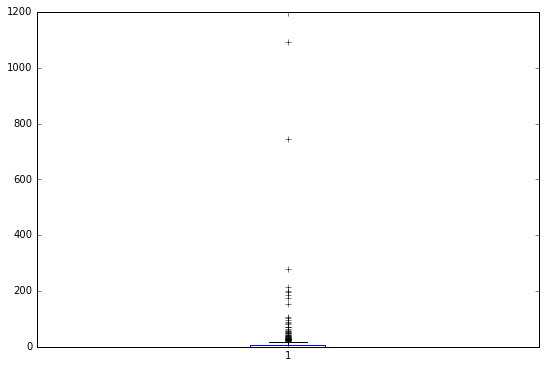
\includegraphics[width=\linewidth]{fig/boxplots/area.png}
\caption{Area}\label{fig:mouse}
\end{subfigure}

\begin{subfigure}[b]{.45\linewidth}
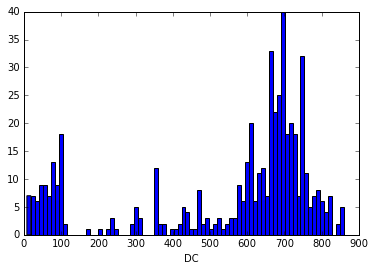
\includegraphics[width=\linewidth]{fig/boxplots/DC.png}
\caption{DC}\label{fig:gull}
\end{subfigure}
\begin{subfigure}[b]{.45\linewidth}
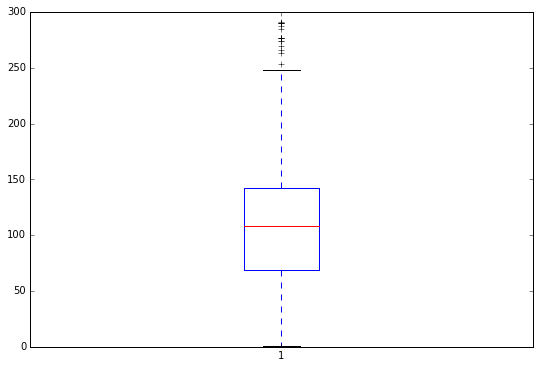
\includegraphics[width=\linewidth]{fig/boxplots/DMC.png}
\caption{DMC}\label{fig:tiger}
\end{subfigure}
\begin{subfigure}[b]{.45\linewidth}
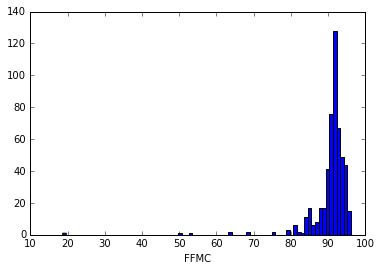
\includegraphics[width=\linewidth]{fig/boxplots/FFMC.png}
\caption{FFMC}\label{fig:tiger}
\end{subfigure}
\begin{subfigure}[b]{.45\linewidth}
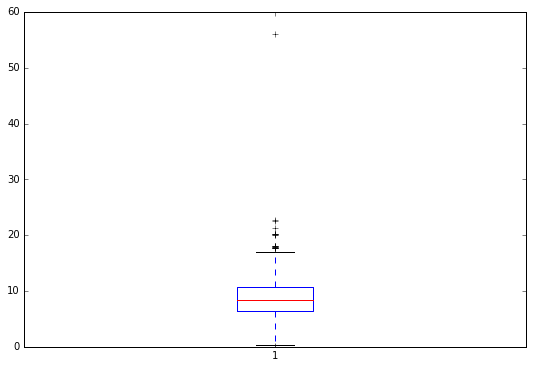
\includegraphics[width=\linewidth]{fig/boxplots/ISI.png}
\caption{ISI}\label{fig:tiger}
\end{subfigure}
%\caption{Picture of animals}
\label{fig:boxplot_1}
\caption{Boxplots 1}
\end{figure}

\begin{figure}[!ht]

\begin{subfigure}[b]{.45\linewidth}
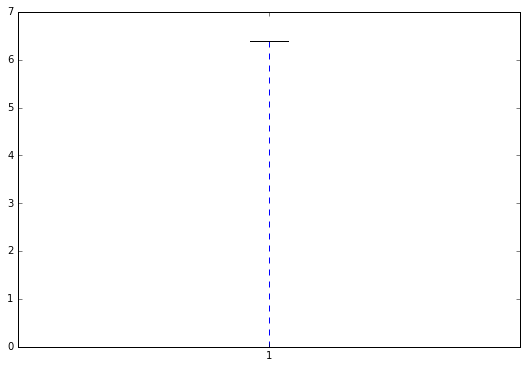
\includegraphics[width=\linewidth]{fig/boxplots/rain.png}
\caption{Rain}\label{fig:mouse}
\end{subfigure}
\begin{subfigure}[b]{.45\linewidth}
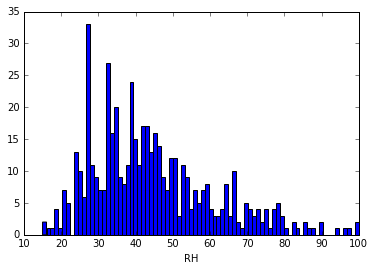
\includegraphics[width=\linewidth]{fig/boxplots/RH.png}
\caption{RH}\label{fig:mouse}
\end{subfigure}
\begin{subfigure}[b]{.45\linewidth}
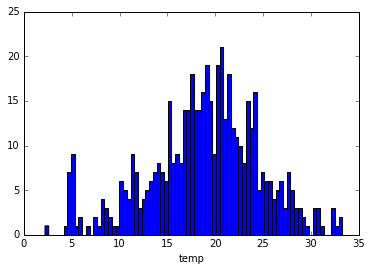
\includegraphics[width=\linewidth]{fig/boxplots/temp.png}
\caption{Temp}\label{fig:gull}
\end{subfigure}
\begin{subfigure}[b]{.45\linewidth}
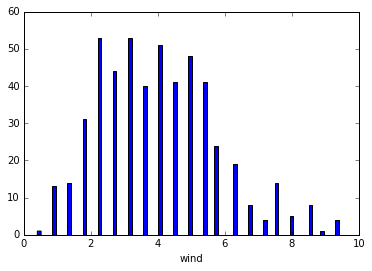
\includegraphics[width=\linewidth]{fig/boxplots/wind.png}
\caption{Wind}\label{fig:tiger}
\end{subfigure}
\begin{subfigure}[b]{.45\linewidth}
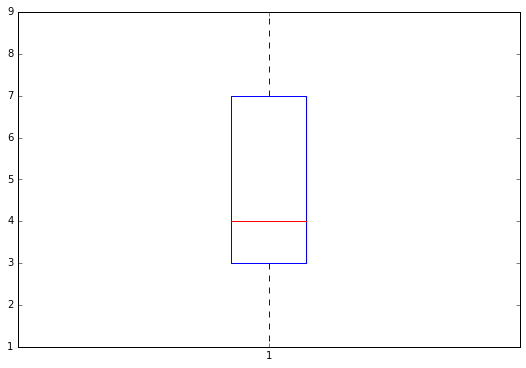
\includegraphics[width=\linewidth]{fig/boxplots/x.png}
\caption{X}\label{fig:tiger}
\end{subfigure}
\begin{subfigure}[b]{.45\linewidth}
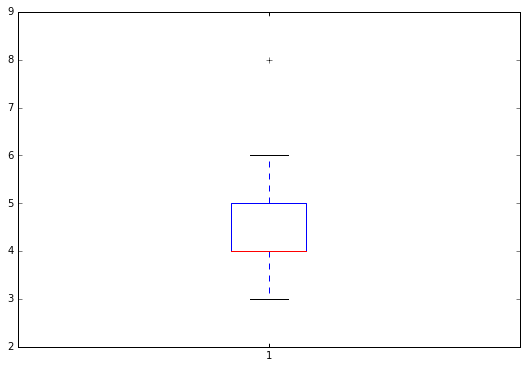
\includegraphics[width=\linewidth]{fig/boxplots/y.png}
\caption{Y}\label{fig:tiger}
\end{subfigure}
\caption{Boxplots 2}
\label{fig:boxplots_2}
\end{figure}